
\chapter{Technical concepts}\label{CCoreConcepts}
Five technical concepts have been developed based on the current solutions, related work and initial tests with the case data:
\begin{itemize}
	\item Load only the needed data
	\item Coloring should be based on the current extent
	\item Tiles should not be precolored
	\item Coloring should be done locally
	\item File format should have same bit depth as input format
\end{itemize}

The purpose of these concepts is to ensure that a large dataset can be loaded and visualized correctly. 

\section{Load only the needed data}
The case data presented in chapter \ref{CCaseData} holds information for the entire world. However, loading data for the entire world would be unnecessarily time consuming. Initial experiments of rendering this quantity of data also revealed that the browser did not have enough memory to load that amount of data. Instead only the relevant data should be downloaded. The relevant data in this case would refer to the data, which the user is able to see. Getting a subset of a raster dataset can be accomplished by dividing it into smaller tiles. 

\section{Coloring should be based on the current extent}\label{ColorFromCurrentExtent}
The initial exploration of the data showed that the coloring of the tiles should be based of the current extent. This is due to how much the values are varying across the world. Figure \ref{WhyLimitToExtent} shows an example of the difference between a map where the coloring is based on all values or if it is limited to the current extent. Both maps illustrate the population in Denmark. The left map has its coloring based on values from the entire world, while the right has its colors based on the current extent. The left map appears to have no population since the population density in Denmark is negligible compared with the most densely populated areas in the world. In the right map it is possible to see the location of the most populated cities. Since the left map provide the user with no relevant information and the right one does, the coloring should be based on the current extent.


\begin{figure} [H]
	\centering
	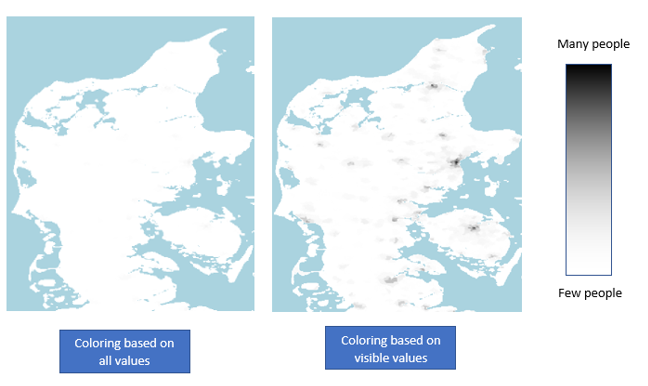
\includegraphics[width=.8\textwidth]{Pictures/WhyLimitToExtent}
	\caption{Population density in Jutland}
	\label{WhyLimitToExtent}
\end{figure}


\section{Tiles should not be precolored}
If the coloring should be based on the current extent and the map is interactive the coloring of the tiles should be done on the fly instead of once and for all. The reason for this is best explained with the example in figure \ref{WhyNotPrecolor}. This figure is illustrating the population in a small subset of India.  The three boxes are illustrating examples of possible map extents, which the user could get by zooming in on different parts of the map. Each of these three have a different max value in their cell with the highest population. The blue square is covering the city center of Indore therefore has a high value than the green, which is covering the outskirts of the city. The last square does not include any part of a bigger city and therefore have a lower value. 
Since their max values are different, they would each need their own coloring. If the tiles were to be precolored it would be necessary to create three coloring of the tiles – one for each the extents. However, since the map is interactive, the extent is not limited to those three. If the user instead were to zoom in on an area between the red and blue square a new max value would maybe be found. When scaling this example up to the entire world and to multiple zoom extents there would be thousands of combinations. If all of these needed to be prerender it would both require lots of initial processing time and storage space for an immense amount of data. 


\begin{figure} [H]
	\centering
	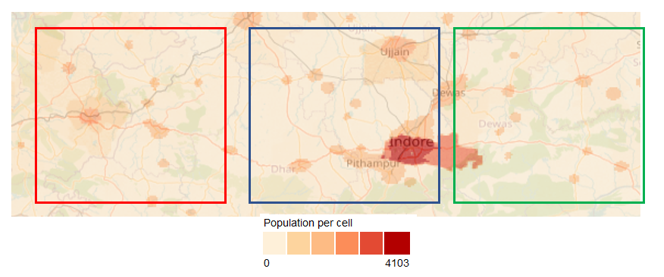
\includegraphics[width=.8\textwidth]{Pictures/WhyNotPrecolor}
	\caption{Population density. The three boxes are examples of possible extents an interacting user could get by zooming.}
	\label{WhyNotPrecolor}
\end{figure}

The alternative is to color the tiles on the fly. When the user would zoom to a new area the map, a script could register the highest currently visible value. This information could then be sent to recoloring script, which would color the tiles based on this. This way only tiles with the needed colors would be rendered. 


\section{Coloring should be done on the client}
The coloring can be done in two ways as illustrated in figure \ref{WhyColorLocally}. It can be done by sending the information to a tileserver, which then would color the tiles and send them to the client. Alternatively, the coloring could be done on the client. 

\begin{figure} [H]
	\centering
	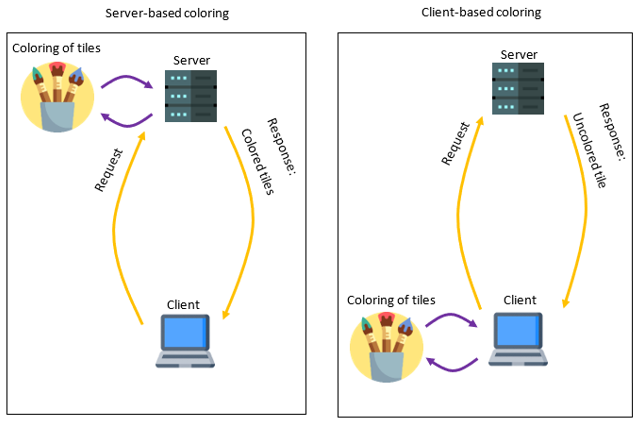
\includegraphics[width=.8\textwidth]{Pictures/WhyColorLocally}
	\caption{Difference between coloring the tile on the server and client. Inspired by a similar looking model from \citet{Baumrocks}. Icon source: \citep{Freepik}}
	\label{WhyColorLocally}
\end{figure}

Comparing the two options is best done with an example, which has been illustrated in figure \ref{WhyColorLocallyMap}. Here the blue and green box are two different possible views both containing 16 raster tiles. The two boxes have different max values, since blue one contains the city center. In the example a user will pan from the blue view to the green one. If the coloring is done on the server side the initial 16 tiles in the blue box will be requested on load.Then when the user pan to the green view the 16 tiles in that box will be requested and colored. The four tiles that are shared between the blue and the green boxes must be requested again, since they need a new color due to the change in max value. This is not the case if the coloring is done locally. In this case only 12 tiles would have to be requested, when changing from the blue to the green view. Since the coloring is happening locally the coloring script can recolor the four tiles it already has downloaded from the initial load.  In the right part of figure \ref{WhyColorLocally} the yellow loop would be run 12 times, whereas the purple one would be run 16 times. This should result in a faster experience for the user.

\begin{figure} [H]
	\centering
	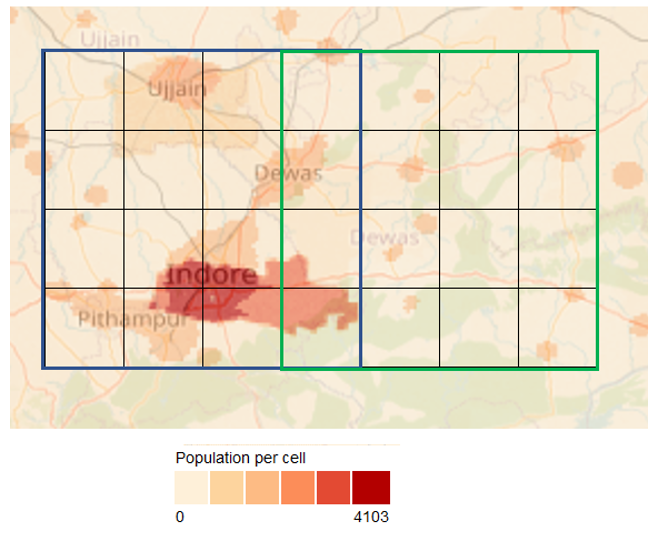
\includegraphics[width=.6\textwidth]{Pictures/WhyColorLocallyMap}
	\caption{Example of why local coloring is needed. The squares are different extents used for the example}
	\label{WhyColorLocallyMap}
\end{figure}

\section{File format should have same bit depth as input format}\label{NeededDepth}
As mention in section x the data from the case has a bit depth of 32 bit. To visualize the data the file format must not be changed to a format with less than 32 bits. Figure \ref{WhyNot8Bit} is an example of how a subset of the case data look originally and when converted to an 8-bit format. As mentioned in section \ref{BitDepth} the pixels in an 8-bit raster can have values between 0-255. This means that this format is unable to correctly display the original data range, where the data range is covering thousands of values. The original data get clamped into the 8-bit format producing wrong result
\citep{gdal2tilesDoc} .

\begin{figure} [H]
	\centering
	\includegraphics[width=.6\textwidth]{Pictures/WhyNot8Bit}
	\caption{32 bits cramped into 8 bits}
	\label{WhyNot8Bit}
\end{figure}

Normally this issue could be worked around by rescaling the input data to the new format \citep{gdal2tilesDoc} . This rescaling would be a lossy compression resulting in loss of information since the original data cannot be expressed with values between 0-255. \citep{Dent}
For the normal use of tiles this would not be a problem since tiles would only be used for visualization. 
If the tiles are being recolored locally the tiles are being used for more than just visualization. It is necessary to access the data within the tile. This means that solutions resulting in a lossy compression are not an option. To ensure that the correct data reach the client the file format used for tiles must have a bit depth of 32.